% \documentclass[dissertation,copyright]{uathesis}
% %DIF LATEXDIFF DIFFERENCE FILE
% %DIF DEL chapter_4_old.tex   Tue Jul 18 10:08:39 2017
% %DIF ADD chapter_4.tex       Wed Jul 26 23:39:30 2017
% \usepackage[]{graphicx}\usepackage[]{color}
% %% maxwidth is the original width if it is less than linewidth
% %% otherwise use linewidth (to make sure the graphics do not exceed the margin)
% \makeatletter
% \def\maxwidth{ %
%   \ifdim\Gin@nat@width>\linewidth
%     \linewidth
%   \else
%     \Gin@nat@width
%   \fi
% }
% \makeatother
% 
% \definecolor{fgcolor}{rgb}{0.345, 0.345, 0.345}
% \newcommand{\hlnum}[1]{\textcolor[rgb]{0.686,0.059,0.569}{#1}}%
% \newcommand{\hlstr}[1]{\textcolor[rgb]{0.192,0.494,0.8}{#1}}%
% \newcommand{\hlcom}[1]{\textcolor[rgb]{0.678,0.584,0.686}{\textit{#1}}}%
% \newcommand{\hlopt}[1]{\textcolor[rgb]{0,0,0}{#1}}%
% \newcommand{\hlstd}[1]{\textcolor[rgb]{0.345,0.345,0.345}{#1}}%
% \newcommand{\hlkwa}[1]{\textcolor[rgb]{0.161,0.373,0.58}{\textbf{#1}}}%
% \newcommand{\hlkwb}[1]{\textcolor[rgb]{0.69,0.353,0.396}{#1}}%
% \newcommand{\hlkwc}[1]{\textcolor[rgb]{0.333,0.667,0.333}{#1}}%
% \newcommand{\hlkwd}[1]{\textcolor[rgb]{0.737,0.353,0.396}{\textbf{#1}}}%
% \let\hlipl\hlkwb
% 
% \usepackage{framed}
% \makeatletter
% \newenvironment{kframe}{%
%  \def\at@end@of@kframe{}%
%  \ifinner\ifhmode%
%   \def\at@end@of@kframe{\end{minipage}}%
%   \begin{minipage}{\columnwidth}%
%  \fi\fi%
%  \def\FrameCommand##1{\hskip\@totalleftmargin \hskip-\fboxsep
%  \colorbox{shadecolor}{##1}\hskip-\fboxsep
%      % There is no \\@totalrightmargin, so:
%      \hskip-\linewidth \hskip-\@totalleftmargin \hskip\columnwidth}%
%  \MakeFramed {\advance\hsize-\width
%    \@totalleftmargin\z@ \linewidth\hsize
%    \@setminipage}}%
%  {\par\unskip\endMakeFramed%
%  \at@end@of@kframe}
% \makeatother
% 
% \definecolor{shadecolor}{rgb}{.97, .97, .97}
% \definecolor{messagecolor}{rgb}{0, 0, 0}
% \definecolor{warningcolor}{rgb}{1, 0, 1}
% \definecolor{errorcolor}{rgb}{1, 0, 0}
% \newenvironment{knitrout}{}{} % an empty environment to be redefined in TeX
% 
% \usepackage{alltt}
% \newcommand{\SweaveOpts}[1]{}  % do not interfere with LaTeX
% \newcommand{\SweaveInput}[1]{} % because they are not real TeX commands
% \newcommand{\Sexpr}[1]{}       % will only be parsed by R
% 
% 
% %\documentclass[dissertation,CC-BY]{uathesis}
% %\documentclass[dissertation,CC-BY-SA]{uathesis}
% %documentclass[dissertation,CC-BY-ND]{uathesis}
% %\documentclass[thesis]{uathesis}
% %\documentclass[document]{uathesis}
% 
% % Package Usage
% % These are the packages that we need
% \usepackage{booktabs}
% \usepackage{graphicx}
% \usepackage{natbib}			% natbib is available on most systems, and is
% 					% terribly handy.
% 					
% %May need to remove! Trying to fix nocite{*} biblography problem:
% 					% If you want to use a different Bibliography package, 
% 					% you should be able to, just change this
% 					% and the \bibliographystyle command below.  Be warned
% 					% that you may need to do a little hacking to get
% 					% the REFERENCES item to show up in your TOC.
% 
% % Compatibility with the AASTEX package 
% % of the American Astronomical Society.
% %\usepackage{deluxetable}		% Allows use of AASTEX deluxe tables
% %\usepackage{aastex_hack}		% Allows other AASTEX functionality.
% 
% % These are other packages that you might find useful.
% % For controlling the fonts, see
% % http://www.math.uiuc.edu/~hartke/computer/latex/survey/survey.html
% % The following is a nice font set:
% %\usepackage{mathtime}			% Times for letters; Belleek math.
% %
% \usepackage{wrapfig}
% %DIF 90-98d90
% %DIF < 
% %DIF < \newenvironment{lydiawrapfigure}
% %DIF <  {%
% %DIF < %  \setlength{\intextsep}{0pt}% <--- Wrong!
% %DIF <   \setlength{\columnsep}{15pt}%
% %DIF <   \wrapfloat{figure}%
% %DIF <  }
% %DIF <  {\endwrapfloat}
% %DIF <  
% %DIF -------
% \usepackage{caption}
% \usepackage{subcaption}
% \usepackage{tipa}
% \usepackage{color,soul}
% \usepackage{url}
% \usepackage{blindtext}
% \usepackage[inline]{enumitem}
% \usepackage{breakurl}
% \usepackage{mathtools}
% %DIF 108c99-126
% %DIF < \usepackage{amsmath}			% AMS Math (advanced math typesetting)
% %DIF -------
% \usepackage{amsmath} %DIF > 
% \usepackage{array} %DIF > 
% \newcolumntype{P}[1]{>{\centering\arraybackslash}p{#1}} %DIF > 
% \newcolumntype{M}[1]{>{\centering\arraybackslash}m{#1}} %DIF > 
%  %DIF > 
% % \usepackage[normalem]{ulem} %DIF > 
% % \usepackage{xyling,comment}			% AMS Math (advanced math typesetting) %DIF > 
% % includecomment{delall} %DIF > 
% % %\excludecomment{delall} %DIF > 
% %  %DIF > 
% % %default: don't show edits %DIF > 
% %  %DIF > 
% % \newcommand{\add}[1]{#1} %DIF > 
% % \newcommand{\del}[1]{} %DIF > 
% % \newcommand{\delni}[1]{} %DIF > 
% % \newcommand{\addtab}{} %DIF > 
% %  %DIF > 
% % %block to show edits controlled by include/exclude-comment above %DIF > 
% % \begin{delall} %DIF > 
% % %added stuff %DIF > 
% % \renewcommand{\add}[1]{\textcolor{blue}{#1}} %DIF > 
% % %added table %DIF > 
% % \renewcommand{\addtab}{\color{blue}} %DIF > 
% % %deleted stuff %DIF > 
% % \renewcommand{\del}[1]{\textcolor{red}{\sout{#1}}} %DIF > 
% % \renewcommand{\delni}[1]{\noindent\textcolor{red}{\sout{#1}}} %DIF > 
% % \end{delall} %DIF > 
%  %DIF > 
% %DIF -------
% %\usepackage{lscape}			% Used for making fitting large tables in by putting them landscape
% %\usepackage{refs}			
% %
% % If you are using hyper-ref (recommended), this command must go after all 
% % other package inclusions (from the hyperref package documentation).
% % The purpose of hyperref is to make the PDF created extensively
% % cross-referenced.
% 
% %Also works! Change dvips to driverfallback=dvips.
% \usepackage[driverfallback=dvips,bookmarks,colorlinks=true,urlcolor=black,linkcolor=black,citecolor=black]{hyperref}
% 
% 
% %Works!
% %\usepackage[pdftex,bookmarks,colorlinks=true,urlcolor=black,linkcolor=black,citecolor=black]{hyperref}
% %HERE IS THE THING THAT NEEDS TO CHANGE TO GET LATEX TO WORK WITH RSTUDIO. USE pdftex instead of dvips.
% 
% % Set up some values.
% \completetitle{Working Title: An approach to automatic and human speech recognition using ear-recorded speech.}
% \fullname{Samuel John Charles Johnston}			% Grad college wants your full name here.
% \degreename{Doctor of Philosophy}	% Title of your degree.
% %DIF PREAMBLE EXTENSION ADDED BY LATEXDIFF
% %DIF UNDERLINE PREAMBLE %DIF PREAMBLE
% \RequirePackage[normalem]{ulem} %DIF PREAMBLE
% \RequirePackage{color}\definecolor{RED}{rgb}{1,0,0}\definecolor{BLUE}{rgb}{0,0,1} %DIF PREAMBLE
% \providecommand{\DIFaddtex}[1]{{\protect\color{blue}\uwave{#1}}} %DIF PREAMBLE
% \providecommand{\DIFdeltex}[1]{{\protect\color{red}\sout{#1}}}                      %DIF PREAMBLE
% %DIF SAFE PREAMBLE %DIF PREAMBLE
% \providecommand{\DIFaddbegin}{} %DIF PREAMBLE
% \providecommand{\DIFaddend}{} %DIF PREAMBLE
% \providecommand{\DIFdelbegin}{} %DIF PREAMBLE
% \providecommand{\DIFdelend}{} %DIF PREAMBLE
% %DIF FLOATSAFE PREAMBLE %DIF PREAMBLE
% \providecommand{\DIFaddFL}[1]{\DIFadd{#1}} %DIF PREAMBLE
% \providecommand{\DIFdelFL}[1]{\DIFdel{#1}} %DIF PREAMBLE
% \providecommand{\DIFaddbeginFL}{} %DIF PREAMBLE
% \providecommand{\DIFaddendFL}{} %DIF PREAMBLE
% \providecommand{\DIFdelbeginFL}{} %DIF PREAMBLE
% \providecommand{\DIFdelendFL}{} %DIF PREAMBLE
% %DIF END PREAMBLE EXTENSION ADDED BY LATEXDIFF
% %DIF PREAMBLE EXTENSION ADDED BY LATEXDIFF
% %DIF HYPERREF PREAMBLE %DIF PREAMBLE
% \providecommand{\DIFadd}[1]{\texorpdfstring{\DIFaddtex{#1}}{#1}} %DIF PREAMBLE
% \providecommand{\DIFdel}[1]{\texorpdfstring{\DIFdeltex{#1}}{}} %DIF PREAMBLE
% %DIF END PREAMBLE EXTENSION ADDED BY LATEXDIFF
% 
% \begin{document}
% %set_parent(‘/Users/mwilli/Documents/Spring_2017/Dissertation_Document/Dissertation_Working_Directory_Draft/Dissertation_Main.Rnw')



 



\chapter{Automatic Speech Recognition of Ear-Recorded Speech\DIFdelbegin %DIFDELCMD < \label{chapter3}%%%
\DIFdelend \DIFaddbegin \label{chapter4}\DIFaddend }


\section{Introduction}\DIFaddbegin \label{chap4:introduction}
\DIFaddend 

The automatic recognition of human speech by a computer has been a subject of interest spanning decades.  Humans first and foremost communicate their ideas via speech and human language, and teaching computers to be able to take verbal instructions would make interaction with them much easier for a majority of the population, particularly the elderly and disabled.  Since this task has been a subject of much study for over half a century, and is only recently gaining much success, it is important to briefly discuss these successes and the challenges that still remain.

%Despite these successes, challenges still remain when there is noise in the signal (\cite{zhang:17}).  As before, it is important to understand the mechanics and acoustics of why this proves to be a challenge for automatic speech recognition (ASR), and traditional methods of dealing with this as well as more modern techniques.

% Insert bit about it being still not perfect?
The present study proposes a new technique to be used in the advancement of noise-robust automatic speech recognition (ASR).
The experiment in Chapter \DIFdelbegin \DIFdel{2}\DIFdelend \ref{chapter2} collected ear-recorded speech data, which aimed to overcome the difficulty of accurately perceiving speech in a noisy environment, for recognition both by computer (ASR) or by human speech perception.  This collected data will be used in an experiment utilizing the standard open-source ASR system Kaldi (\cite{povey:11}) with the standard, freely-available acoustic model developed from the LibriSpeech corpus (\cite{panayotov:15}).

\section{Background}
\DIFdelbegin %DIFDELCMD < \label{chap3:background}
%DIFDELCMD < %%%
\DIFdelend \DIFaddbegin \label{chap4:background}
\DIFaddend 

% Things to hit on:
% - Base-level Acoustics-to-Features
% - Traditional general ASR mechanics?
% - Current methods of ASR (Cutajar + more recent)
% - Outline problem of noise in the signal
% - Traditional methods of filtering noise out of the signal
% - Previous methods of ASR in noise
% -- Issues with these traditional methods (of removing noise and ASR in noise)
% - Current methods of ASR in noise (Li 2014, and more current)
% -- Multiple Microphones and Beamforming
% -- Other methods??  Look at current CHiME challenge papers
% - Try to find continued issue with electronically identifying speech in noise
% - Emphasize unpredictability of noise, and unknown amplitude - how ear-recorded speech may be able to `protect' against this unpredicatability

%DIF <  The basics of the acoustics of speech was discussed at the beginning of Chapter 2\ref{chapter2}.  As a recap, speech contains voiced and voiceless sounds.  The voiceless sounds are generally produced by turbulence - air moving rapidly through a small openning in the vocal tract.  The voiced sounds are more complex, and contain harmonics (acoustic energy focused in very narrow bands of frequency).  Certain harmonics (out of the full set of harmonics in the voiced signal) contain more energy than the other harmonics; these regions in the frequency spectrum with harmonics containing greater energy are called formants, and this is where much of the speech information comes from.
%DIF >  The basics of the acoustics of speech was discussed at the beginning of Chapter \ref{chapter2}.  As a recap, speech contains voiced and voiceless sounds.  The voiceless sounds are generally produced by turbulence - air moving rapidly through a small openning in the vocal tract.  The voiced sounds are more complex, and contain harmonics (acoustic energy focused in very narrow bands of frequency).  Certain harmonics (out of the full set of harmonics in the voiced signal) contain more energy than the other harmonics; these regions in the frequency spectrum with harmonics containing greater energy are called formants, and this is where much of the speech information comes from.
% 
% The human auditory system does a remarkable job of finding these acoustic features and interpreting them, but a computer does not have an inherent auditory system and (as of now) needs to be told what to look for.  Simply put, via a microphone, computers receive a series of digits (numbers) which correspond to the amount of pressure at a given point in time.  
% %
% \begin{wrapfigure}{L}{0.5\textwidth}
% \centering
% 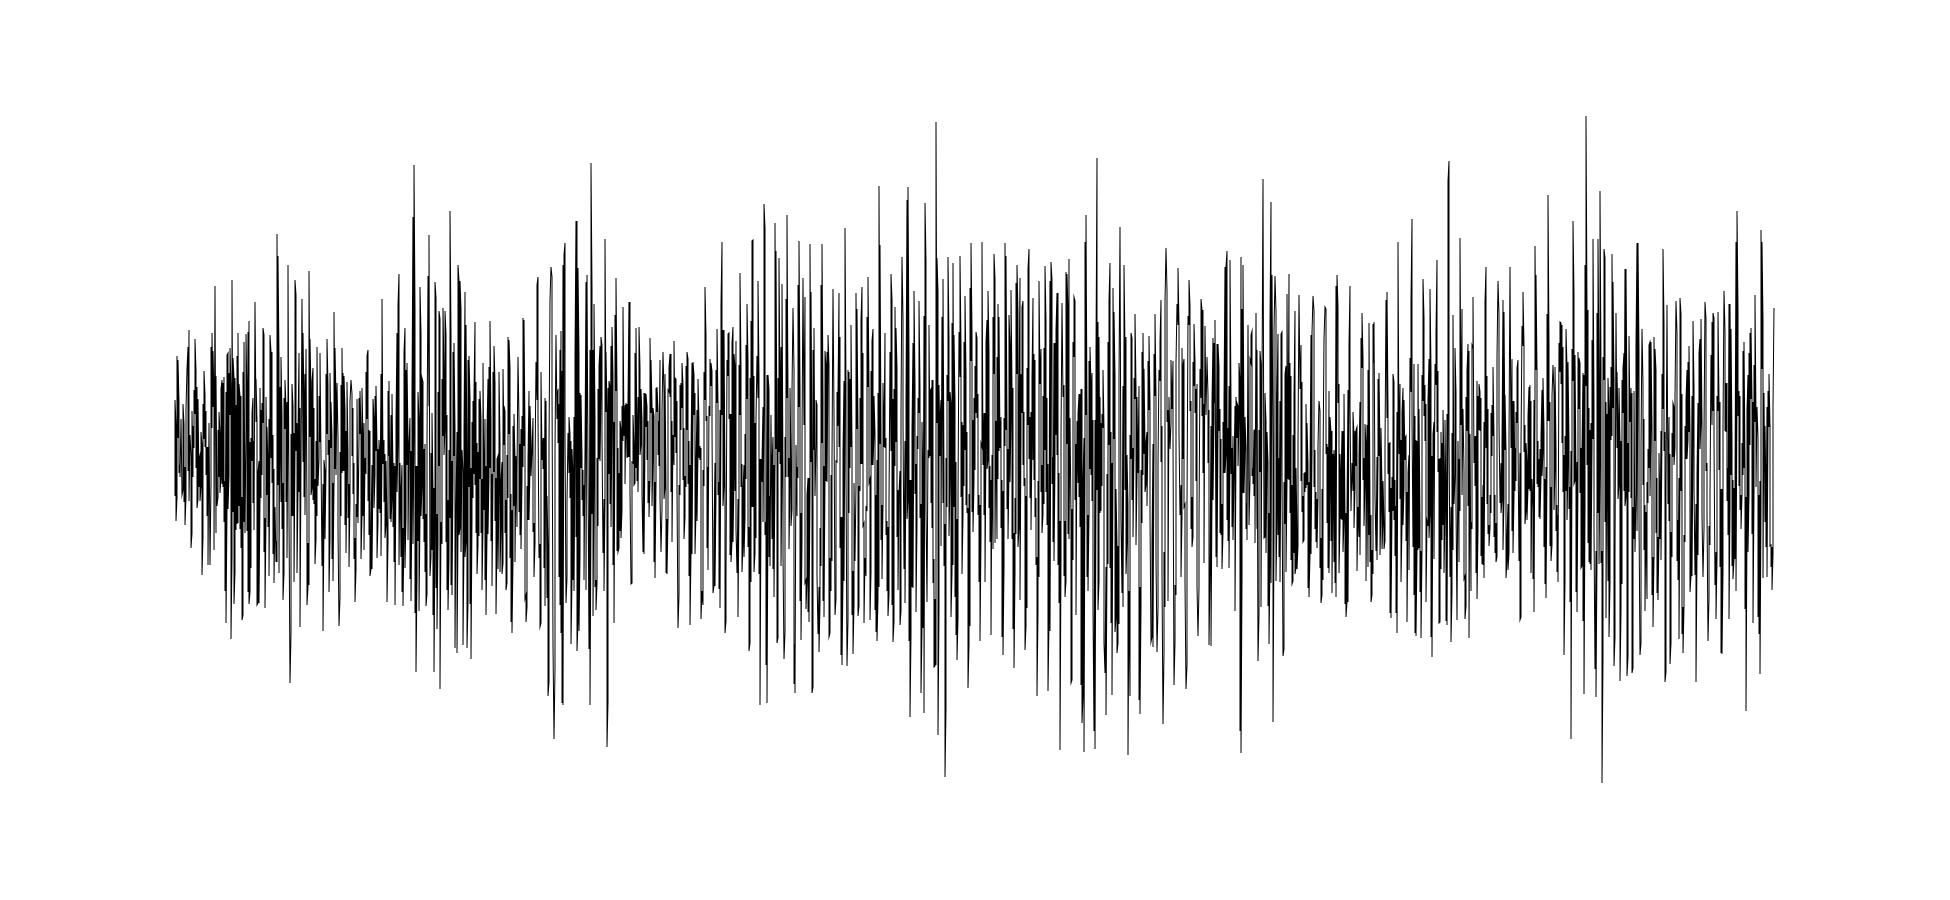
\includegraphics[width=0.45\textwidth]{figure/single-channel-animals.png}
%   \caption{A waveform graph representing the high and low pressure fluctuations that comprise sound.}
%   \label{fig:waveform}
% \end{wrapfigure}

While there are more than 30 years of research involving ASR, and nearly as many working with speech in noisy environments, it is impossible to mention all or even most developed techniques within this very brief overview.  Therefore, the discussion will involve only several areas of research in noise-robust ASR that pertain to the present study.

Equation \ref{eq:basic} is often used to represent the combination of speech and noise,
\begin{equation}\label{eq:basic}
x * h + n = y
\end{equation}
where $x$ is the clean speech signal, $h$ is any convolution (eg. room reverberation, microphone channel warp, etc.) of the original speech signal, $n$ is additive noise, and $y$ is the noisy speech signal.  In addition, the phase of the component signals contributing to the resulting signal $y$ also has an effect.  Taking phase into account means that additive noise is not always simply additive, as energy at frequencies with competing phases could cancel each other out to varying degrees, depending on phase.  While there is some research that does take phase into account and demonstrates that by doing so, more accurate noise removal can be achieved, attempting to model phase adds significant complexity, and the - albeit problematic (many researchers admit) - assumption is frequently made that phase plays no role (\cite{li:14}).  

%Multi-style training, what it is (training with multiple types of noise) - it is ineffective.  Older - paper cited was written in 1987. \cite{li:14}, \cite{lippmann:87}.

The categorization of noise-robustness techniques utilized by hundreds of researchers over the years is difficult, but, broadly, two domains can be outlined (\cite{li:14,zhang:17}).  The first is the \DIFdelbegin \DIFdel{``}\DIFdelend \DIFaddbegin \DIFadd{`}\DIFaddend feature-space\DIFdelbegin \DIFdel{'' }\DIFdelend \DIFaddbegin \DIFadd{' }\DIFaddend domain, which focuses on front-end processing of the signal $y$ itself.  The second group utilizes the \DIFdelbegin \DIFdel{``model space'' }\DIFdelend \DIFaddbegin \DIFadd{`model-space' }\DIFaddend domain, or the back-end processing that modifies the acoustic model to account for any noise in the signal $y$.  Feature space is the part of the ASR process where an acoustic vector is transformed into `features' describing salient parts the acoustic signal that the ASR model will receive as input.  Model space, consequently, then, comes after feature space in the ASR process, and encompasses the acoustic model parameters, methods of training the model, etc.  

Noise can be accounted for in either the feature space domain or the model space domain, or both.  In the feature domain, noise is dealt with, and the signal is enhanced, prior to sending the features to the acoustic model for recognition.  These modifications are made without altering the acoustic model parameters, resulting in low computation cost.  In the model space, acoustic parameters themselves can be modified in accordance with the noisy signal.  This generally results in high computation cost when training the acoustic model.  There is normally a trade-off between the two domains: one of computation efficiency and performance. Model space alterations often yielding higher performance improvement, while feature space alterations are less computationally intensive (\cite{li:14}).
Advances in neural network technology have also lent itself to application in noise-robust ASR.  These have provided additional methods of tackling the problem.

\subsection{Feature Space Domain}

In the feature space domain of noise-robust ASR processing, there are a number of broad techniques, including (a) noise-resistant features, (b) feature normalization, and  (c) feature compensation.  Noise resistant features are, quite simply, features in the acoustic signal which are not sensitive to environmental changes.  Many researchers have proposed many methods of signal derivation that incorporate features of the human auditory system, including Perceptual Linear Prediction (PLP, \cite{hermansky:85}), introducing the \DIFdelbegin \DIFdel{``auditory spectrum'' }\DIFdelend \DIFaddbegin \DIFadd{`auditory spectrum' }\DIFaddend and explicit formant information into ASR processing, and Relative Spectral processing (RASTA) applied to PLP (\cite{hermansky:92}), making PLP less sensitive to slow varying speech information and more sensitive to the more rapid-varying transitions of speech, which is important in human speech perception (\cite{willi:17}).  \cite{kim:99} attempts to model functions of the cochlea and auditory nerve. These methods are quite effective at dealing with short-term, stationary, additive noise (\cite{zhang:17}).  More recent methods include SPARK (\cite{fazel:12}, 1369), which is ``neurobiologically inspired'' by ``auditory receptive fields'' and ``local competitive behavior'', and that proposed by \cite{moritz:15}, which emulates the amplitude modulation found in mammalian auditory cortexes.  These are just a selection of methods incorporating biologically based noise resistant features, which generally outperform \DIFdelbegin \DIFdel{``vanilla'' }\DIFdelend \DIFaddbegin \DIFadd{`vanilla' }\DIFaddend MFCC methods. The fact that these features can be quite complex to generate, and the parameters difficult to set, makes it hard to utilize a combination of them, preventing widespread usage and incorporation with other techniques.  A straightforward relation between the cleaned features and noisy speech is also difficult to derive due to the complexity involved in the feature calculation (\cite{li:14}).

Feature normalization (b) generally involves normalizing cepstral feature vectors in the form of cepstral mean normalization (CMN) and cepstral mean and variance normalization (CMVN).  CMN involves finding the mean values out of all cepstral vectors (\cite{atal:74}).  All cepstral vectors are then normalized, such that the mean cepstral value becomes zero.  CMN primarily eliminates reverberation and channel-related distortion, but signals with noise and no channel distortion also see improvement (\cite{droppo:08}).  CMVN takes the mean and normalizes it together with the co-variance of the cepstral vectors, yielding improved performance on speech data with additive noise (\cite{viikki:98}).
These methods do not work in real-time, however, as they require cepstral vectors from the entire utterance in order to calculate means and variances.

Feature compensation (c) actually attempts to remove the noise from the noisy speech signal, allowing for use of traditional features. Spectral subtraction (\cite{boll:79} is an intuitive method of removing noise by taking a small window of the waveform, turning the linear signal into the spectral domain, and subtracting an existing or estimated noise spectrum $n$ from a noisy speech spectrum $y$, leaving a spectrum of clean speech $x$.  This is then converted back into the time domain, and the process is repeated all along the waveform.  Spectral subtraction often estimates the noise by looking at sections of the observed signal that do not contain speech information.  

This method still has several problems (\cite{li:14}). First and foremost, the location of speech in the signal in a noisy environment is difficult to detect, which consequently affects the ability to accurately compute a noise average. It also requires relatively stationary, slow-variation noise; noise that changes quickly can have a different average spectrum during the portion of the signal containing speech than the portion of the signal in which the noisy spectrum was calculated.  Furthermore, this is only an average of the noise, and not exactly the noise itself.  This subtraction of the average can inadvertently have an additive noise effect by producing extraneous acoustic artifacts in the \DIFdelbegin \DIFdel{``clean'' }\DIFdelend \DIFaddbegin \DIFadd{`clean' }\DIFaddend signal which were not there to begin with (\cite{berouti:79}).

Wiener filtering (\cite{lim:79}) is another method used to remove noise from a signal.  As opposed to spectral subtraction, however, this is a linear filter that works without the need to convert the signal into spectra.  However, this method also requires an estimation of the noise.  Furthermore, it does not do well in very low SNR environments, as it generally results in suppression and dampening of the entire signal, and not just the noise (\cite{li:14}).

More standard, is the \DIFdelbegin \DIFdel{``}\DIFdelend \DIFaddbegin \DIFadd{`}\DIFaddend advanced front-end\DIFdelbegin \DIFdel{'' }\DIFdelend \DIFaddbegin \DIFadd{' }\DIFaddend (AFE) ensemble proposed in \cite{etsi:02}.  It yields more than 50\% improvement over standard MFCC features alone, and has become a frequent baseline for comparison in noisy ASR research.  It is composed of three separate `tools': two-stage Mel-warped Wiener filtering, SNR-dependent waveform processing, and blind equalization (cf. \cite{agarwal:99,macho:02,macho:01,mauuary:98}).

Most of the heavy work of the AFE ensemble is performed by the Mel-warped Wiener filtering (\cite{agarwal:99,li:14}).  This filter differs from the more standard Wiener filter in that it uses the Mel-frequency power spectrum in the Wiener filter calculations, as opposed to the linear signal, the result of which is then converted back into the time domain.  The filter is applied once, and then a second time to remove residual noise.  SNR-dependent waveform processing (SDWP, \cite{macho:01}) assumes that the noise remains relatively constant, whereas the speech signal causes variation in the amplitude of the signal.  SDWP uses this assumption to dampen portions of the signal with a relatively constant and low SNR compared with the high SNR (ie, speech-less versus speech-bearing) portions of the signal, which are amplified.  Blind equalization serves to eliminate convolutional (eg. reverberant) distortion from the signal (\cite{mauuary:98}).

Considered to be the best \DIFdelbegin \DIFdel{``general purpose'' }\DIFdelend \DIFaddbegin \DIFadd{`general-purpose' }\DIFaddend noise-removal tool (\cite{zhang:17}, 4) using traditional (non-neural network) techniques, the minimum mean square error (MMSE) magnitude modulation estimator (MME) was developed by \cite{paliwal:12}, and based on the acoustic modulation estimator (AME) first proposed by \cite{ephraim:84}.  The approach utilizes the spectral modulation magnitude domain, rather than the spectral frequency domain (as is used in the AME method), which is where much of its success originates.

\subsection{Feature Space Domain: Neural Networks}

Broadly, there are two primary categories of utilizing neural networks to account for noisy speech: \DIFdelbegin \DIFdel{``mapping methods'' and ``masking methods'' }\DIFdelend \DIFaddbegin \DIFadd{`mapping methods' and `masking methods' }\DIFaddend (\cite{zhang:17}).  Mapping methods involve finding the non-linear function that maps the noisy speech to the clean speech.  In neural network terms, the noisy speech is the input to some type of neural network (eg. Deep Neural Network (NN), Convolutional NN, Recurrent NN, etc.) and the (intended) output is an approximation of the clean speech.  Due to the complexity of speech in the temporal domain, the input to the neural network usually comes from one of the higher-processed input transformations, such as from the spectral or cepstral domains.

Masking-based approaches work similarly to a traditional filter, albeit learned via a neural network. A method using an `Ideal Ratio Mask' will use a neural network to learn the ratio (value between 0 and 1) of the presence of clean speech to noise.  %The neural network then ``learns'' this masking ratio value that can be applied to the noisy speech signal $y$ to ideally return the clean speech $x$ as output.  
This process is most beneficial when using spectral or cepstral features as inputs.  These calculated masking ratio values are then multiplied element-wise to each spectral or cepstral feature (from the noisy signal $y$) at every time index, returning the estimation of the clean speech $x$ as output (\cite{zhang:17}).


% Model Space
\subsection{Model Space Domain}

The description of model space domain compensation techniques will be brief, as this is not the focus of the present study.  This form of compensation usually involves adapting an existing acoustic model (presumably trained on relatively clean speech) to enable recognition of more noisy features.  Variations of maximum likelihood linear regression (MLLR, \cite{leggetter:95}) are often used to adjust the %gaussian component vector 
model means and co-variance parameters to account for differences in the signal that is introduced by noise.  There are many variations and extensions of MLLR; one such variation, feature-space MLLR, or fMLLR, actually moves MLLR application into the feature domain (\cite{gales:98}).  

There are also a few model-based approaches using neural networks for noise-robust ASR.  Most widely used is multi-condition training (\cite{seltzer:13,zhang:17}), which, similar to multi-style training originally developed by \cite{lippman:87}, uses a collection of training data that exhibits a wide range of noise conditions.  Another technique, similar to methods used in non-neural network approaches, involves adapting the already trained acoustic model with a small subset of noisy data.  However, as doing so can inadvertently result in significant overfitting, \cite{mirsamadi:15} have developed a technique unique to neural networks that - instead of slightly adjusting all weights, adds an additional layer to the neural network with its own weights.  This largely avoids the issue of overfitting, while increasing the model's robustness to noise.

\cite{weninger:13}, among many others, also combine the modifications in the feature space domain with modifications in the model space domain, referred to as joint model training.  Broadly, this takes the form of using the feature-based noise removal techniques to output feature-enhanced data which is then used as training data itself for the acoustic model.

\subsection{Microphone Arrays}

There are also techniques that employ multiple microphones as a method of source-separation to extract the speech source from any extraneous noise sources. Beamforming (\cite{veen:88}), for example, has become a central technique to using microphone arrays for source separation (\cite{hori:15,zhang:17}).
The direction of arrival of the different sound sources is calculated, taking into account the distance between the two (or more) microphones, and the time of arrival of the different sources in each signal recorded by each microphone.  Recent work (cf. \cite{heymann:15,sivasankaran:15,heymann:16}) has also employed neural networks to aid and enhance the beamforming process . 

\subsection{Summary}

Most research over the past few decades has focused on feature space domain modifications.  This is likely due to the intensive computation required by many model space domain techniques.  Leading feature-space techniques include MMSE-MME (\cite{paliwal:12}) and AFE (\cite{etsi:02}). %which is often used as a standard baseline for comparison with new feature space modifications.  
Model space domain approaches include adjusting the acoustic model parameters, often using a form of MLLR (\cite{leggetter:95}), which can also take the form of fMLLR in the feature space domain.  In the last few years, the advent of neural networks has seen further improvement in both feature and model space domains.  Other recent approaches have combined feature and model space modifications (joint model training), and the use of multiple microphones into a microphone input array has also become more mainstream. The recent CHiME challenges (\cite{chime:16}) have incorporated the use of multi-channel ASR input as well as single channel input as part of its task.

Most of these employed feature and model space techniques that are used to account for noise are still forced to make estimations about noise type, SNR, and noise location in the signal.  As would be expected, as SNR decreases, and as noise becomes more variable (non-stationary), these methods begin to falter.  Chapter \DIFdelbegin \DIFdel{2\ref{chapter2} proposes }\DIFdelend \DIFaddbegin \DIFadd{\ref{chapter2} proposed }\DIFaddend a method of collecting speech in noisy environments (recording speech from the inside of the ear canal) that is hypothesized to be largely immune to noise type and the stationarity (or lack thereof) of noise.  It does not require any noise estimation or inference.  It would be classified as a form of feature-space modification, affecting the signal in the temporal domain before it even reaches the microphone.  The only drawback encountered is that the speech in the recorded signal is heavily low-pass filtered, where the highest speech frequencies observed in the signal are generally found near 2.7 kHz.

The only processing performed after the signal is recorded is pre-emphasis and low-pass filtering, which could be easily built into the recording mechanism itself.  It is hypothesized that this method of passive noise removal via recording speech from the ear canal, plus the minimal modification of pre-emphasis and low-pass filtering, will demonstrate similar gains over noisy speech achieved by many of the other techniques described above.


% Another tool used is the exploitation of any prior knowledge about the distortion (\cite{li:14}); this is prior knowledge that is utilized during the training stage, not knowledge about the noise during the testing stage.  Some methods include learning the mapping between noisy and non-noisy pairs of acoustic signals.  This mapping is then extended to novel noisy utterances during testing.  This is used in feature domain space to enhance a noisy speech feature to then send to the model.  
% 
% Other methods utilze mutliple acoustic models, each trained on data from different environments and different noises and different SNRs.  The means and covariance matrices of each of these models are stored, and during recognition, the most appropriate model is chosen to use to decode the signal in question.  Either of these tactics, though, do require prior knowledge about the noise.  As with multi-style training, explained above, it is very difficult to ensure that all noises, SNRs, etc, are adequately accounted for during training in order to be prepared for what is seen during testing.
% 
% 
% %Implicit vs Explicit Distortion Modelling
% 
% Explicit distortion modelling uses a ``physical model'' which allows for high performance with few distortion parameters. An example of an explicit distortion model would be spectral subtraction, discussed earlier.  It seems obvious that spectral subtraction, when matched with an agreeable signal that best utilizes its noise removal abilities, would result in more accurate speech recognition.  Consequently, other noise reduction methods that \textit{explicitly} specify the distortion tend to perform well.
%
%
% \textbf{For examples of what this distortion model actually is, go to the primary literature:}
% Y. Zhao and B. H. Juang, “A comparative study of noise estimation
% algorithms for VTS-based robust speech recognition,” in
% Proc. Inter-
% speech
% , 2010, pp. 2090–2093.
% J.Li,L.Deng,D.Yu,Y.Gong,
% andA.Acero,“Hi
% gh-performance
% HMM adaptation with joint compensation of additive and convolutive
% distortions via vector Taylor series,” in
% Proc. ASRU
% , 2007, pp. 65–70.
% [132] J.Li,L.Deng,D.Yu,Y.Gong,andA.Acero,“Auni
% fi
% ed framework of
% HMM adaptation with joint compensation of additive and convolutive
% distortions,”
% Comput., Speech, Lang.
% , vol. 23, no. 3, pp. 389–405, 2009.






 




% For noise-robust ASR utilizing multiple microphones, refer to any of the following:
% T.Virtanen,R.Singh,andB.Raj
% , Techniques for noise robustness in
% automatic speech recognition
% .  New York, NY, USA: Wiley, 2012. OR
% 
% [31] S. Makino, T.-W. Lee, and H. Sawada
% , Blind Speech Separation
% .
% New York, NY, USA: Springer, 2007.
% [32] J. Benesty, M. M. Sondhi, and Y. Huang
% , Springer Handbook of Speech
% Processing
% .  New York, NY, USA: Springer, 2007.
% [33] P. A. Naylor and N. D. Gaubitch
% , Speech Dereverberation
% .New
% York, NY, USA: Springer, 2010.
% 
% ALSO
% 
% [41] T. Yoshioka and T. Nakatani, “Noise model transfer: Novel approach
% to robustness against nonstationary noise,”
% IEEE Trans. Audio, Speech,
% Lang. Process.
% , vol. 21, no. 10, pp. 2182–2192, Oct. 2013
% 
% AND
% 
% [42] M.Souden,S.Araki,K.Kinoshita,T.Nakatani,andH.Sawada,“A
% multichannel mmse-based framework for speech source separation and
% noise reduction,”
% IEEE Trans. Audio, Speech, Lang. Process.
% ,vol.21,
% no. 9, pp. 1913–1928, Sep. 2013.





\DIFdelbegin %DIFDELCMD < \section{Experiment 2: ASR of Ear-Recorded and Noisy Mouth-Recorded Speech}
%DIFDELCMD < %%%
\DIFdelend \DIFaddbegin \section{Experiment 3: ASR of Ear-Recorded and Noisy Mouth-Recorded Speech}\label{expt3}
\DIFaddend 

While there are many proposed techniques, discussed in Section \DIFdelbegin \DIFdel{\ref{chap3:background}}\DIFdelend \DIFaddbegin \DIFadd{\ref{chap4:background}}\DIFaddend , that have been used to modify the acoustic features of noisy speech, or to modify the acoustic model to compensate for noise, noise-robust ASR is still imperfect and requires additional advances to ASR technology (\cite{zhang:17}).  This particular study proposes the new technique of using speech recorded from the inside of the ear canal.  This would be classified as a feature space modification in the temporal domain, prior to any processing.  Rather than using significant computation to achieve the noise reduction, this study employs purely passive mechanisms (ie. tissues in the head, earplug, \DIFdelbegin \DIFdel{ear muffs}\DIFdelend \DIFaddbegin \DIFadd{earmuffs}\DIFaddend ) to reduce noise.  

As described previously in Chapter \DIFdelbegin \DIFdel{2}\DIFdelend \ref{chapter2}, very simple signal enhancement techniques (ie. pre-emphasis and band-pass filtering)\footnote{These are simple enough to be hard-wired into an electrical chip to be performed in real-time, requiring no actual computation.} are then applied to the recorded signal to produce an enhanced signal with relatively little noise and one that is very similar (below 2.7 kHz) to what could be recorded at the mouth \DIFaddbegin \DIFadd{in absence of noise}\DIFaddend .

\subsection{Stimuli}
\DIFaddbegin \label{chap4:methods:stimuli}
\DIFaddend 

Recordings from twenty speakers, ten male and ten female, from the data collection experiment in Chapter \DIFdelbegin \DIFdel{2\ref{chapter2} comprises }\DIFdelend \DIFaddbegin \DIFadd{\ref{chapter2} comprised }\DIFaddend the test data for this experiment.  This included 30 distinct sentences from each speaker, each with 5 different noise conditions (bus, cafe, pedestrian, street, factory) with 3 different noise levels (60dB, 70dB, 80dB), plus an additional `clean' (no noise) condition.  This \DIFdelbegin \DIFdel{results }\DIFdelend \DIFaddbegin \DIFadd{resulted }\DIFaddend in 16 iterations of each distinct sentence (30), for each microphone location (2), \DIFdelbegin \DIFdel{resulting }\DIFdelend \DIFaddbegin \DIFadd{which resulted }\DIFaddend in 960 utterances for each of 20 speakers, totaling 19200 test utterances.  There \DIFdelbegin \DIFdel{are }\DIFdelend \DIFaddbegin \DIFadd{were }\DIFaddend 9600 ear-recorded utterances (6 hours, 55 minutes)\footnote{Time estimates are calculated from an average utterance duration of ~2.6 seconds}, 9000 mouth-recorded noisy utterances (6 hours, 30 minutes), and 600 mouth-recorded clean utterances (26 minutes).

Two additional datasets were used.  One was recorded from the mouth with the intention to obtain speech with a lower SNR - described in Chapter \DIFdelbegin \DIFdel{4\ref{chapter4}, Section \ref{chap4:methods:stimuli}}\DIFdelend \DIFaddbegin \DIFadd{\ref{chapter3}, Section \ref{chap3:methods:stimuli}}\DIFaddend .  The other was the dataset (recorded at the same time) of ear signals combined with the mouth signals from the dataset above; the low-frequency ear-recorded signal was combined with the high-frequency components of the mouth-recorded signal, described in Chapter \DIFdelbegin \DIFdel{4\ref{chapter4}}\DIFdelend \DIFaddbegin \DIFadd{\ref{chapter3}}\DIFaddend , Section \ref{F0-methods}.
For these two datasets, each contained two speakers, one male and one female.  The dataset of speech combined from ear- and mouth-recorded signals contains 80 distinct utterances, each repeated 5 times (the `clean' speech condition was removed) by each of 2 speakers, totaling 800 utterances.  The dataset of speech recorded at the mouth in noisy conditions contains 80 distinct utterances, each repeated 5 times (again, the `clean' speech condition was removed) by each of 2 speakers, totaling 800 utterances.  These datasets were recorded simultaneously at the ear and at the mouth, from the same two speakers.

\DIFdelbegin %DIFDELCMD < \subsection{Design}
%DIFDELCMD < %%%
\DIFdelend \DIFaddbegin \subsection{Design and Procedure}
\label{chap4:methods:design}
\DIFaddend 

The existing deep neural network (DNN) acoustic model trained on 960 hours of speech from the LibriSpeech corpus (published and described in \cite{panayotov:15}) was used to test the collected data.  As described in \cite{panayotov:15}, the 960 hours of data, collected from the audio transcripts of books from the LibriVox website, was divided into two groups - `clean' and `other'.  This designation was chosen by preliminarily running an acoustic model trained on Wall Street Journal data (WSJ, \cite{paul:92}) on the LibriSpeech utterances. The set was split down the middle, with the half containing lower WERs designated at the `clean' set, and those with higher WERs designated as the `other' set.  Data from both sets were used in training the LibriSpeech acoustic model.

Additionally, the ASR setup utilized the language models from \cite{panayotov:15}, trained on the LibriSpeech corpus.  To verify the current set-up of the acoustic and language models, the \DIFdelbegin \DIFdel{experimenter }\DIFdelend \DIFaddbegin \DIFadd{author }\DIFaddend performed a replication of \cite{panayotov:15}'s experiment using LibriSpeech's \DIFdelbegin \DIFdel{``}\DIFdelend \DIFaddbegin \DIFadd{`}\DIFaddend test-clean\DIFdelbegin \DIFdel{'' and ``}\DIFdelend \DIFaddbegin \DIFadd{' and `}\DIFaddend test-other\DIFdelbegin \DIFdel{'' }\DIFdelend \DIFaddbegin \DIFadd{' }\DIFaddend datasets.  Afterwards, the \DIFdelbegin \DIFdel{experimenter used the the }\DIFdelend same acoustic and language models \DIFaddbegin \DIFadd{were used }\DIFaddend to recognize the speech data collected for this study described in Chapter \DIFdelbegin \DIFdel{2}\DIFdelend \ref{chapter2}. This primarily tested the performance between the ear-recorded and noisy mouth-recorded speech, but also between the different noise conditions and noise levels.  The \DIFdelbegin \DIFdel{experimenter }\DIFdelend \DIFaddbegin \DIFadd{author }\DIFaddend also tested the data collected for, and described in \DIFdelbegin \DIFdel{Chater 4\ref{chapter4}}\DIFdelend \DIFaddbegin \DIFadd{Chapter \ref{chapter3}}\DIFaddend , containing very noisy mouth-recorded data and the data combination of mouth- and ear-recorded speech.
%DIF < It is likely that, due to the ear-recorded speech only containing information below 3 kHz, that the existing acoustic model in its current state will have poor recognition of these sentences, and quite possibly will not outperform the noisy speech using the LibriSpeech models, particularly due to the relatively high SNR noisy speech.  
\DIFaddbegin \DIFadd{It is likely that, due to the ear-recorded speech only containing information below 3 kHz, that the existing acoustic model in its current state will have poor recognition of these sentences, and quite possibly will not outperform the noisy speech using the LibriSpeech models, particularly due to the relatively high SNR noisy speech.
}

\DIFadd{A common method of improving ASR performance on speech with different characteristics (eg. in noise, with different dialects, etc.) is to train the ASR acoustic model on speech in that domain.  This also mimics the process utilized by the human auditory system to `adapt' its acoustic model to better recognize an adverse condition using `training'; this was used in the human speech perception task described in Chapter \ref{chapter3} and Section \ref{sec:chap3-review}.  Rather than recording enough ear-recorded speech to train a model, the a subset of 75 hours of the 100-hour dataset from the LibriSpeech corpus was used.  The speech in this dataset was lowpassed with the exact same filter used on the ear-recorded speech - 2.5 kHz with a 500 Hz slope.  A speaker-adapted GMM-HMM model was trained on this data.  Due to resource constraints, computationally and otherwise, only the subset of the 100-hour dataset was used (not 960 hour), and a DNN model was not trained from the GMM model.
}

\DIFadd{Furthermore, the ear-recorded stimuli were modified for a final test.  This combined the pre-emphasized, ear-recorded speech, which is lowpass filtered to 2.5 kHz with a 500 Hz slope, with the simultaneous speech recorded at the mouth, which was bandpass filtered from 3.0 kHz to 8.0 kHz, with a 500 Hz slope in either direction}\footnote{\DIFadd{The mouth-recorded speech was already lowpass filtered to 8.0 kHz.}}\DIFadd{. This same transformation was performed on the ear-recorded stimuli for a follow-up human speech perception task in Chapter \ref{chapter3}.  The motivation behind this transformation is that it will re-introduce some high-frequency speech information which is not present in the ear-recorded signal alone.
}\DIFaddend 

%Due to this assumption, 


%Both the ear-recorded and noisy mouth data will then be enhanced using the well-established advanced front end (AFE, \cite{etsi:02}) technique, and will be retested on the same, unchanged acoustic model.

%DIF < A common practice in ASR research is to use a relatively small subset of data to adapt an existing acoustic model to better fit the style of data currently being used.  As additional training was used on a subset of human listeners in the experiment in Chapter 4\ref{chapter4} Section \ref{}, this training will be used in an attempt to modify the acoustic model to better recognize the ear-recorded speech.  The same DNN LibriSpeech acoustic model will be adapted with ear-recorded, low-pass filtered additional utterances (not from the 30 test sentences, nor from any of the speakers being tested).  A total of 50 distinct sentences repeated in 5 noise conditions from 4 additional speakers were used for adaptation of the acoustic model, totalling 1000 utterances used for adaptation.  The total duration of these utterances combined is approximately 44 minutes. The same 19200 utterances from the same 20 speakers were used again as test data.
%DIF > A common practice in ASR research is to use a relatively small subset of data to adapt an existing acoustic model to better fit the style of data currently being used.  As additional training was used on a subset of human listeners in the experiment in Chapter 3\ref{chapter3} Section \ref{}, this training will be used in an attempt to modify the acoustic model to better recognize the ear-recorded speech.  The same DNN LibriSpeech acoustic model will be adapted with ear-recorded, low-pass filtered additional utterances (not from the 30 test sentences, nor from any of the speakers being tested).  A total of 50 distinct sentences repeated in 5 noise conditions from 4 additional speakers were used for adaptation of the acoustic model, totalling 1000 utterances used for adaptation.  The total duration of these utterances combined is approximately 44 minutes. The same 19200 utterances from the same 20 speakers were used again as test data.



\subsection{Results}
\DIFaddbegin \label{chap4:results}
\DIFaddend 

\DIFdelbegin \DIFdel{The experimenter used }\DIFdelend LibriSpeech test data \DIFdelbegin \DIFdel{on the configured }\DIFdelend \DIFaddbegin \DIFadd{was used on the existing }\DIFaddend acoustic and language models specified above \DIFaddbegin \DIFadd{to verify the Kaldi ASR system was configured correctly}\DIFaddend .  Table \ref{tab:sanity-check} demonstrates that accuracy \DIFdelbegin \DIFdel{similar to }\DIFdelend \DIFaddbegin \DIFadd{near }\DIFaddend the published results was achieved, and the acoustic and language model \DIFdelbegin \DIFdel{set up }\DIFdelend \DIFaddbegin \DIFadd{set-up }\DIFaddend was verified.

\begin{table}[h]
\begin{center}
\begin{tabular}{| c || c | c | c | c |} \hline
Language Models & Clean Publ. & Clean Repl. & Other Publ. & Other Repl. \\ \hline\hline
3-gram, thresh. 3e-7 & 8.02 & 9.15 & 19.41 & 23.76 \\ \hline
3-gram, thresh. 1e-7 & 7.21 & 8.20 & 17.66 & 21.55 \\ \hline
3-gram, unpruned & 5.74 & 6.50 & 14.77 & 18.37 \\ \hline
4-gram, unpruned & 5.51 & 6.20 & 13.97 & 17.53 \\ \hline
\end{tabular}
\end{center}
\caption{The `Language Models' column specifies the Language Model (LM) used in each row; two LMs are simply the 3-gram model which was pruned to the specified threshold.  `Publ.' columns list the performance listed in the published paper, and `Repl.' columns contain the replication performance achieved in the present study.  `Clean' and `Other' refer to the clean (2707 utterances) and `noisy' (5968 utterances) LibriSpeech test datasets. All LMs utilize the 960-hour LibriSpeech DNN acoustic model.  All values are given as WER.}\label{tab:sanity-check}
\end{table}

The \DIFdelbegin \DIFdel{experimenter }\DIFdelend \DIFaddbegin \DIFadd{author }\DIFaddend then used data collected in the present study, described in Chapter \DIFdelbegin \DIFdel{2}\DIFdelend \ref{chapter2} with the same acoustic and language models.  Table \ref{tab:basic-run} shows these results.  This table combines all noisy speech at the mouth into a single `Noisy Mouth' category and all speech collected at the ear into a single `Ear Speech' category.

\begin{table}[h]
\begin{center}
\begin{tabular}{| c || c | c | c |} \hline
Language Models & Clean Mouth & Noisy Mouth & Ear Speech \\ \hline\hline
3-gram, prune thresh. 3e-7 & 16.74 & 51.04 & 84.10 \\ \hline
3-gram, prune thresh. 1e-7 & 14.01 & 49.11 & 83.55 \\ \hline
3-gram, unpruned & 9.52 & 44.49 & 82.29 \\ \hline
4-gram, unpruned & 9.38 & 44.31 & 82.47 \\ \hline
\end{tabular}
\end{center}
\caption{The `Language Models' column specifies the Language Model (LM) used in each row; two LMs are simply the 3-gram model which was pruned to the specified threshold.  \DIFdelbeginFL \DIFdelFL{``}\DIFdelendFL \DIFaddbeginFL \DIFaddFL{`}\DIFaddendFL Clean Mouth\DIFdelbeginFL \DIFdelFL{'' }\DIFdelendFL \DIFaddbeginFL \DIFaddFL{' }\DIFaddendFL includes only the sentences recorded at the mouth with no noise, versus \DIFdelbeginFL \DIFdelFL{``}\DIFdelendFL \DIFaddbeginFL \DIFaddFL{`}\DIFaddendFL Noisy Mouth\DIFdelbeginFL \DIFdelFL{''}\DIFdelendFL \DIFaddbeginFL \DIFaddFL{'}\DIFaddendFL , which includes all other [noisy] sentences recorded at the mouth. \DIFdelbeginFL \DIFdelFL{``}\DIFdelendFL \DIFaddbeginFL \DIFaddFL{`}\DIFaddendFL Ear Speech\DIFdelbeginFL \DIFdelFL{'' }\DIFdelendFL \DIFaddbeginFL \DIFaddFL{' }\DIFaddendFL contains all ear-recorded utterances.  All LMs utilize the 960-hour LibriSpeech DNN acoustic model.  All values are given as WER.}\label{tab:basic-run}
\end{table}

\DIFaddbegin \DIFadd{A simple comparison of clean mouth-recorded speech and the simultaneous (clean) ear-recorded speech is located in Table \ref{tab:clean-wers}.
}

\begin{table}[h]
\begin{center}
\begin{tabular}{| c | c |} \hline
 \DIFaddFL{Mouth-Recorded, Clean }& \DIFaddFL{Ear-Recorded, Clean }\\ \hline\hline
 \DIFaddFL{9.38 }& \DIFaddFL{79.30 }\\ \hline
\end{tabular}
\end{center}
\caption{\DIFaddFL{A comparison of ASR performance on mouth-recorded speech and ear-recorded speech with no background noise. These values are obtained from the highest-performing (4-gram) language model, utilizing the 960-hour LibriSpeech DNN acoustic model - both trained using the LibriSpeech corpus.  All values are give as WER.}}\label{tab:clean-wers}
\end{table}

\DIFaddend Table \ref{tab:split-wer-noise} separates out the noisy mouth-recorded speech \DIFdelbegin \DIFdel{into its }\DIFdelend \DIFaddbegin \DIFadd{and ear-recorded speech into the }\DIFaddend different noise types and noise levels.

\begin{table}[h]
\begin{center}
\DIFdelbeginFL %DIFDELCMD < \begin{tabular}{| c || c | c | c | c | c || c |} %%%
\DIFdelendFL \DIFaddbeginFL \begin{tabular}{| c || c | c | c | c | c | c | c | c | c | c | c | c |} \DIFaddendFL \hline
      &  \multicolumn{2}{|c|}{Bus}  &  \multicolumn{2}{|c|}{Cafe}  &  \multicolumn{2}{|c|}{Ped.}  &  \multicolumn{2}{|c|}{Street} \DIFaddendFL &  \multicolumn{2}{|c|}{Factory}  \\ \hline
      & \DIFdelbeginFL \DIFdelFL{Totals }\DIFdelendFL \DIFaddbeginFL \DIFaddFL{Mth }& \DIFaddFL{Ear }& \DIFaddFL{Mth }& \DIFaddFL{Ear }& \DIFaddFL{Mth }& \DIFaddFL{Ear }& \DIFaddFL{Mth }& \DIFaddFL{Ear }& \DIFaddFL{Mth }& \DIFaddFL{Ear }\DIFaddendFL \\ \hline\hline
60 dB & \DIFdelbeginFL \DIFdelFL{21.51 }\DIFdelendFL \DIFaddbeginFL \DIFaddFL{21.5 }\DIFaddendFL & \DIFdelbeginFL \DIFdelFL{20.33 }\DIFdelendFL \DIFaddbeginFL \DIFaddFL{81.1 }\DIFaddendFL & \DIFdelbeginFL \DIFdelFL{18.64 }\DIFdelendFL \DIFaddbeginFL \DIFaddFL{20.3 }\DIFaddendFL & \DIFdelbeginFL \DIFdelFL{19.05 }\DIFdelendFL \DIFaddbeginFL \DIFaddFL{82.1 }\DIFaddendFL & \DIFdelbeginFL \DIFdelFL{17.93 }\DIFdelendFL \DIFaddbeginFL \DIFaddFL{18.6 }\DIFaddendFL & \DIFdelbeginFL \textbf{\DIFdelFL{19.49}} %DIFAUXCMD
\DIFdelendFL \DIFaddbeginFL \DIFaddFL{81.5 }& \DIFaddFL{19.0 }& \DIFaddFL{81.4 }& \DIFaddFL{17.9 }& \DIFaddFL{80.6  }\DIFaddendFL \\ \hline
70 dB & \DIFdelbeginFL \DIFdelFL{41.74 }\DIFdelendFL \DIFaddbeginFL \DIFaddFL{41.7 }\DIFaddendFL & \DIFdelbeginFL \DIFdelFL{32.93 }\DIFdelendFL \DIFaddbeginFL \DIFaddFL{81.8 }\DIFaddendFL & \DIFdelbeginFL \DIFdelFL{32.02 }\DIFdelendFL \DIFaddbeginFL \DIFaddFL{32.9 }\DIFaddendFL & \DIFdelbeginFL \DIFdelFL{36.49 }\DIFdelendFL \DIFaddbeginFL \DIFaddFL{80.6 }\DIFaddendFL & \DIFdelbeginFL \DIFdelFL{29.96 }\DIFdelendFL \DIFaddbeginFL \DIFaddFL{32.0 }\DIFaddendFL & \DIFdelbeginFL \textbf{\DIFdelFL{34.63}} %DIFAUXCMD
\DIFdelendFL \DIFaddbeginFL \DIFaddFL{82.7 }& \DIFaddFL{36.4 }& \DIFaddFL{82.0 }& \DIFaddFL{29.9 }& \DIFaddFL{81.8  }\DIFaddendFL \\ \hline
80 dB & \DIFdelbeginFL \DIFdelFL{88.20 }%DIFDELCMD < & %%%
\DIFdelFL{73.39 }%DIFDELCMD < & %%%
\DIFdelFL{75.64 }\DIFdelendFL \DIFaddbeginFL \DIFaddFL{88.2 }\DIFaddendFL & \DIFdelbeginFL \DIFdelFL{85.00 }\DIFdelendFL \DIFaddbeginFL \DIFaddFL{83.0 }\DIFaddendFL & \DIFdelbeginFL \DIFdelFL{71.43 }\DIFdelendFL \DIFaddbeginFL \DIFaddFL{73.3 }\DIFaddendFL & \DIFdelbeginFL \textbf{\DIFdelFL{78.73}} %DIFAUXCMD
%DIFDELCMD < \\ \hline\hline
%DIFDELCMD < %%%
\DIFdelFL{Totals }\DIFdelendFL \DIFaddbeginFL \DIFaddFL{82.6 }\DIFaddendFL & \DIFdelbeginFL \textbf{\DIFdelFL{50.48}} %DIFAUXCMD
\DIFdelendFL \DIFaddbeginFL \DIFaddFL{75.6 }\DIFaddendFL & \DIFdelbeginFL \textbf{\DIFdelFL{42.22}} %DIFAUXCMD
\DIFdelendFL \DIFaddbeginFL \DIFaddFL{85.0 }\DIFaddendFL & \DIFdelbeginFL \textbf{\DIFdelFL{42.10}} %DIFAUXCMD
\DIFdelendFL \DIFaddbeginFL \DIFaddFL{85.0 }\DIFaddendFL & \DIFdelbeginFL \textbf{\DIFdelFL{46.85}} %DIFAUXCMD
\DIFdelendFL \DIFaddbeginFL \DIFaddFL{85.7 }\DIFaddendFL & \DIFdelbeginFL \textbf{\DIFdelFL{39.77}} %DIFAUXCMD
\DIFdelendFL \DIFaddbeginFL \DIFaddFL{71.4 }\DIFaddendFL & \DIFdelbeginFL \textbf{\DIFdelFL{44.28}\footnote{\DIFdelFL{This value differs slightly to the joint noise WER value given in Table \ref{tab:basic-run}, but the difference can be attributed to rounding estimations.}}%DIFAUXCMD
\addtocounter{footnote}{-1}%DIFAUXCMD
} %DIFAUXCMD
\DIFdelendFL \DIFaddbeginFL \DIFaddFL{85.0 }\DIFaddendFL \\ \hline
\end{tabular}
\end{center}
\caption{These \DIFaddbeginFL \DIFaddFL{values }\DIFaddendFL are \DIFdelbeginFL \DIFdelFL{only }\DIFdelendFL \DIFaddbeginFL \DIFaddFL{obtained }\DIFaddendFL from the highest-performing (4-gram) language model, utilizing the 960-hour LibriSpeech DNN acoustic model \DIFaddbeginFL \DIFaddFL{- both trained using the LibriSpeech corpus}\DIFaddendFL .  Each row is a different noise level, and each column a different noise type (excluding the `clean' noise type)\DIFdelbeginFL \DIFdelFL{.  Totals (averages) for }\DIFdelendFL \DIFaddbeginFL \DIFaddFL{, with }\DIFaddendFL each \DIFdelbeginFL \DIFdelFL{category are given in the bottom-most row and }\DIFdelendFL \DIFaddbeginFL \DIFaddFL{sub-column comparing }\DIFaddendFL the \DIFdelbeginFL \DIFdelFL{right-most column}\DIFdelendFL \DIFaddbeginFL \DIFaddFL{performance on mouth-recorded speech in that condition with ear-recorded speech in that condition}\DIFaddendFL .  All values are given as WER.}\label{tab:split-wer-noise}
\end{table}
%DIF >  \begin{table}[h]
%DIF >  \begin{center}
%DIF >  \begin{tabular}{| c || c | c | c | c | c | c | c | c | c | c | c | c |} \hline
%DIF >        & \multicolumn{2}{|c|}{Bus} & \multicolumn{2}{|c|}{Cafe} & \multicolumn{2}{|c|}{Ped.} & \multicolumn{2}{|c|}{Street} & \multicolumn{2}{|c|}{Factory} \\ \hline
%DIF >        & Mth & Ear & Mth & Ear & Mth & Ear & Mth & Ear & Mth & Ear \\ \hline\hline
%DIF >  60 dB & 21.5 & 81.18 & 20.3 & 82.17 & 18.6 & 81.55 & 19.0 & 81.43 & 17.9 & 80.66  \\ \hline
%DIF >  70 dB & 41.7 & 81.88 & 32.9 & 80.66 & 32.0 & 82.71 & 36.4 & 82.05 & 29.9 & 81.82  \\ \hline
%DIF >  80 dB & 88.2 & 83.08 & 73.3 & 82.62 & 75.6 & 85.00 & 85.0 & 85.72 & 71.4 & 85.02 \\ \hline
%DIF >  \end{tabular}
%DIF >  \end{center}
%DIF >  \caption{These values are obtained from the highest-performing (4-gram) language model, utilizing the 960-hour LibriSpeech DNN acoustic model - both trained using the LibriSpeech corpus.  Each row is a different noise level, and each column a different noise type (excluding the `clean' noise type), with each subcolumn comparing the performance on mouth-recorded speech in that condition with ear-recorded speech in that condition.  All values are given as WER.}\label{tab:split-wer-noise}
%DIF >  \end{table}
%DIF >  \begin{table}[h]
%DIF >  \begin{center}
%DIF >  \begin{tabular}{| c || c | c | c | c | c || c |} \hline
%DIF >   & Bus & Cafe & Pedestrian & Street & Factory & Totals \\ \hline\hline
%DIF >  60 dB & 21.51 & 20.33 & 18.64 & 19.05 & 17.93 & \textbf{19.49} \\ \hline
%DIF >  70 dB & 41.74 & 32.93 & 32.02 & 36.49 & 29.96 & \textbf{34.63} \\ \hline
%DIF >  80 dB & 88.20 & 73.39 & 75.64 & 85.00 & 71.43 & \textbf{78.73} \\ \hline\hline
%DIF >  Totals & \textbf{50.48} & \textbf{42.22} & \textbf{42.10} & \textbf{46.85} & \textbf{39.77} & \textbf{44.28} \\ \hline
%DIF >  \end{tabular}
%DIF >  \end{center}
%DIF >  \caption{These are only from the highest-performing (4-gram) language model, utilizing the 960-hour LibriSpeech DNN acoustic model.  Each row is a different noise level, and each column a different noise type (excluding the `clean' noise type).  Totals (averages) for each category are given in the bottom-most row and the right-most column.  The overall average differs slightly from the joint noise WER value given in Table \ref{tab:basic-run}, but the difference can be attributed to rounding estimations. All values are given as WER.}\label{tab:split-wer-noise}
%DIF >  \end{table}

\DIFdelbegin \DIFdel{The experimenter performed another test using two sets of data created in Chapter 4\ref{chapter4}.  One includes the very noisy speech collected for the experiment in Chapter 4\ref{chapter4}}\DIFdelend %DIF >  The experimenter performed another test using two sets of data created in Chapter \ref{chapter3}.  One includes the very noisy speech collected for the experiment in Chapter \ref{chapter3}.  This speech was re-recorded in a way that resulted in a lower SNR; for more details, refer to Section \ref{chap3:methods:stimuli}.    
%DIF >  
%DIF >  
%DIF >  \begin{table}[h]
%DIF >  \begin{center}
%DIF >  \begin{tabular}{| c || c | c |} \hline
%DIF >  Language Models & Ear/Mouth Combined & Extra Noisy Mouth \\ \hline\hline
%DIF >  3-gram, prune thresh. 3e-7 & 85.18 & 98.32 \\ \hline
%DIF >  3-gram, prune thresh. 1e-7 & 84.66 & 99.14 \\ \hline
%DIF >  3-gram, unpruned & 84.04 & 99.03 \\ \hline
%DIF >  4-gram, unpruned & 83.90 & 99.41 \\ \hline
%DIF >  \end{tabular}
%DIF >  \end{center}
%DIF >  \caption{The `Language Models' column specifies the Language Model (LM) used in each row; two LMs are simply the 3-gram model which was pruned to the specified threshold.  The `Ear/Mouth Combined' column contains the results from the dataset using speech reconstructed from low-frequency ear-signal and high frequency mouth-signal parts.  The `Extra Noisy Mouth' column contains results from the re-recorded mouth speech (described in Section \ref{chap3:methods:stimuli}), with a lower SNR.  Note that the data used in these tests are different than those used in previous tests displayed in Tables \ref{tab:basic-run} and \ref{tab:split-wer-noise}. All LMs utilize the 960-hour LibriSpeech DNN acoustic model.  All values are given as WER.}\label{tab:follow-up-asr}
%DIF >  \end{table}
\DIFaddbegin 

%DIF > After retraining the 
%DIF >  The other data set combined the low-passed ear-recorded speech (approximately 0-2.7 kHz) with the very noisy speech from the same utterance, high-pass filtered from approximately 2.7 kHz to 8 kHz.  The WER results are given in Table \ref{tab:follow-up-asr}.

\DIFadd{A new model was trained using a 75-hour subset of the 100-hour portion of the LibriSpeech training corpus}\DIFaddend .  This speech was \DIFdelbegin \DIFdel{re-recorded in a way that resulted in a lower SNR; for more details, refer to Section \ref{chap4:methods:stimuli}.  }\DIFdelend \DIFaddbegin \DIFadd{lowpass filtered at 2.5 kHz with a 500 Hz slope - the same filtering applied to the ear-recorded speech.  A GMM-HMM acoustic model was trained using the LibriSpeech training recipe for Kaldi.  A larger training set was not used - and a neural-net-based acoustic model was not trained - due to computational resource limitations.  The basic performance of this model on the pre-emphasized and filtered ear-recorded speech is given in Table \ref{tab:retrainedGMM}
}\DIFaddend 

\begin{table}[h]
\begin{center}
\DIFdelbeginFL %DIFDELCMD < \begin{tabular}{| c || c | c |} %%%
\DIFdelendFL \DIFaddbeginFL \begin{tabular}{|c||p{2cm}|p{2cm}|p{2cm}|p{2cm}|} \DIFaddendFL \hline
 Language Models & \DIFdelbeginFL \DIFdelFL{Ear/Mouth Combined }%DIFDELCMD < & %%%
\DIFdelFL{Extra Noisy Mouth }%DIFDELCMD < \\ \hline\hline
%DIFDELCMD < %%%
\DIFdelendFL 3-gram, prune thresh. 3e-7 & \DIFdelbeginFL \DIFdelFL{85.18 }%DIFDELCMD < & %%%
\DIFdelFL{98.32 }%DIFDELCMD < \\ \hline
%DIFDELCMD < %%%
\DIFdelendFL 3-gram, prune thresh. 1e-7 & \DIFdelbeginFL \DIFdelFL{84.66 }%DIFDELCMD < & %%%
\DIFdelFL{99.14 }%DIFDELCMD < \\ \hline
%DIFDELCMD < %%%
\DIFdelendFL 3-gram, unpruned & \DIFdelbeginFL \DIFdelFL{84.04 }%DIFDELCMD < & %%%
\DIFdelFL{99.03 }%DIFDELCMD < \\ \hline
%DIFDELCMD < %%%
\DIFdelendFL 4-gram, unpruned \DIFaddbeginFL \\ \hline\hline
 \DIFaddFL{Ear Speech Performance }\DIFaddendFL & \DIFdelbeginFL \DIFdelFL{83.90 }\DIFdelendFL \DIFaddbeginFL \DIFaddFL{92.5 }\DIFaddendFL & \DIFdelbeginFL \DIFdelFL{99.41 }\DIFdelendFL \DIFaddbeginFL \DIFaddFL{92.5 }& \DIFaddFL{92.5 }& \DIFaddFL{92.8 }\DIFaddendFL \\ \hline
\end{tabular}
\end{center}
\caption{The \DIFdelbeginFL \DIFdelFL{`Language Models' column specifies the Language Model (LM) used in each row; two LMs are simply }\DIFdelendFL \DIFaddbeginFL \DIFaddFL{performance obtained from }\DIFaddendFL the \DIFdelbeginFL \DIFdelFL{3-gram }\DIFdelendFL \DIFaddbeginFL \DIFaddFL{acoustic }\DIFaddendFL model \DIFaddbeginFL \DIFaddFL{trained on 75-hours of mouth-recorded speech }\DIFaddendFL which \DIFdelbeginFL \DIFdelFL{was pruned }\DIFdelendFL \DIFaddbeginFL \DIFaddFL{had been lowpass filtered }\DIFaddendFL to \DIFdelbeginFL \DIFdelFL{the specified threshold.  The `Ear/Mouth Combined' column contains the results from the dataset using speech reconstructed from low-frequency ear-signal and high frequency mouth-signal parts.  The `Extra Noisy Mouth' column contains results from the re-recorded mouth speech (described in Section \ref{chap4:methods:stimuli}), }\DIFdelendFL \DIFaddbeginFL \DIFaddFL{2.5 kHz }\DIFaddendFL with a \DIFdelbeginFL \DIFdelFL{lower SNR.  Note that the data used in these tests are different than those used in previous tests displayed in Tables \ref{tab:basic-run} and \ref{tab:split-wer-noise}. All LMs utilize the 960-hour LibriSpeech DNN acoustic model}\DIFdelendFL \DIFaddbeginFL \DIFaddFL{500 Hz slope}\DIFaddendFL .  All values are \DIFdelbeginFL \DIFdelFL{given as }\DIFdelendFL \DIFaddbeginFL \DIFaddFL{in }\DIFaddendFL WER.}\DIFdelbeginFL %DIFDELCMD < \label{tab:follow-up-asr}
%DIFDELCMD < %%%
\DIFdelendFL \DIFaddbeginFL \label{tab:retrainedGMM}
\DIFaddendFL \end{table}

%DIF < After retraining the 
\DIFdelbegin \DIFdel{The other data set combined the low-passed }\DIFdelend \DIFaddbegin \DIFadd{A final test was performed which manipulated the }\DIFaddend ear-recorded \DIFdelbegin \DIFdel{speech (approximately 0-2.7 kHz ) with the very noisy speech from the same utterance, high-pass filtered from approximately 2.7 kHz to 8 kHz.  The WER results are given in Table \ref{tab:follow-up-asr}}\DIFdelend \DIFaddbegin \DIFadd{signal by adding a bandpass-filtered mouth recorded signal (3.0-8.0 kHz with a 500Hz slope) to the lowpass-filtered ear-recorded signal.  This `hybrid' signal was tested using the original DNN acoustic model trained on 960-hour LibriSpeech data.  The results are presented in Table \ref{tab:hybrid-wers} alongside the noisy mouth-recorded speech for comparison (the mouth-recorded results already appeared in Table \ref{tab:split-wer-noise}).  The hybrid ear-recorded data is labeled as `E/M'.
}

\begin{table}[h]
\begin{center}
\begin{tabular}{| c || c | c | c | c | c | c | c | c | c | c | c | c |} \hline
      & \multicolumn{2}{|c|}{Bus} & \multicolumn{2}{|c|}{Cafe} & \multicolumn{2}{|c|}{Ped.} & \multicolumn{2}{|c|}{Street} & \multicolumn{2}{|c|}{Factory} \\ \hline
      & \DIFaddFL{Mth }& \DIFaddFL{E/M }& \DIFaddFL{Mth }& \DIFaddFL{E/M }& \DIFaddFL{Mth }& \DIFaddFL{E/M }& \DIFaddFL{Mth }& \DIFaddFL{E/M }& \DIFaddFL{Mth }& \DIFaddFL{E/M }\\ \hline\hline
\DIFaddFL{60 dB }& \DIFaddFL{21.5 }& \DIFaddFL{52.7 }& \DIFaddFL{20.3 }& \DIFaddFL{51.1 }& \DIFaddFL{18.6 }& \DIFaddFL{52.2 }& \DIFaddFL{19.0 }& \DIFaddFL{51.3 }& \DIFaddFL{17.9 }& \DIFaddFL{51.8  }\\ \hline
\DIFaddFL{70 dB }& \DIFaddFL{41.7 }& \DIFaddFL{58.8 }& \DIFaddFL{32.9 }& \DIFaddFL{54.3 }& \DIFaddFL{32.0 }& \DIFaddFL{55.1 }& \DIFaddFL{36.4 }& \DIFaddFL{56.1 }& \DIFaddFL{29.9 }& \DIFaddFL{53.4  }\\ \hline
\DIFaddFL{80 dB }& \DIFaddFL{88.2 }& \DIFaddFL{78.7 }& \DIFaddFL{73.3 }& \DIFaddFL{70.0 }& \DIFaddFL{75.6 }& \DIFaddFL{71.8 }& \DIFaddFL{85.0 }& \DIFaddFL{74.2 }& \DIFaddFL{71.4 }& \DIFaddFL{71.5  }\\ \hline
\end{tabular}
\end{center}
\caption{\DIFaddFL{These values are obtained from the highest-performing (4-gram) language model, utilizing the 960-hour LibriSpeech DNN acoustic model - both trained using the LibriSpeech corpus.  Each row is a different noise level, and each column a different noise type (excluding the `clean' noise type), with each sub-column listing the performance of mouth-recorded speech (Mth) or `hybrid' ear-recorded speech (E/M) in the same condition.  All values are given as WER.}}\label{tab:hybrid-wers}
\end{table}
%DIF >  \begin{table}[h]
%DIF >  \begin{center}
%DIF >  \begin{tabular}{| c || c | c | c | c | c | c | c | c | c | c | c | c |} \hline
%DIF >        & \multicolumn{2}{|c|}{Bus} & \multicolumn{2}{|c|}{Cafe} & \multicolumn{2}{|c|}{Ped.} & \multicolumn{2}{|c|}{Street} & \multicolumn{2}{|c|}{Factory} \\ \hline
%DIF >        & Mth & E/M & Mth & E/M & Mth & E/M & Mth & E/M & Mth & E/M \\ \hline\hline
%DIF >  60 dB & 21.5 & 52.77 & 20.3 & 51.16 & 18.6 & 52.23 & 19.0 & 51.38 & 17.9 & 51.82  \\ \hline
%DIF >  70 dB & 41.7 & 58.80 & 32.9 & 54.30 & 32.0 & 55.10 & 36.4 & 56.16 & 29.9 & 53.49  \\ \hline
%DIF >  80 dB & 88.2 & 78.78 & 73.3 & 70.04 & 75.6 & 71.82 & 85.0 & 74.21 & 71.4 & 71.51  \\ \hline
%DIF >  \end{tabular}
%DIF >  \end{center}
%DIF >  \caption{These values are obtained from the highest-performing (4-gram) language model, utilizing the 960-hour LibriSpeech DNN acoustic model - both trained using the LibriSpeech corpus.  Each row is a different noise level, and each column a different noise type (excluding the `clean' noise type), with each sub-column listing the performance of mouth-recorded speech (Mth) or `hybrid' ear-recorded speech (E/M) in the same condition.  All values are given as WER.}\label{tab:hybrid-wers}
%DIF >  \end{table}

\DIFadd{These tables demonstrate that, in all but a few noisy conditions, an ASR system will more easily recognize noisy speech than it will ear-recorded speech}\DIFaddend .  




\section{Discussion}
\DIFaddbegin \label{chap4:discussion}
\DIFaddend 

The results indicate, broadly, that the ear-recorded speech (\DIFdelbegin \DIFdel{cf. Table \ref{tab:basic-run}) (}\DIFdelend which has been pre-emphasized and low-pass filtered $<$ 2.7 kHz) performs\DIFaddbegin \DIFadd{, at best, }\DIFaddend minimally better than \DIFdelbegin \DIFdel{two of the 80dB noise conditions - the bus and street background noises }\DIFdelend \DIFaddbegin \DIFadd{only the bus noise type in 80 dB background noise }\DIFaddend (cf. \DIFdelbegin \DIFdel{Tables \ref{tab:basic-run} and }\DIFdelend \DIFaddbegin \DIFadd{Table }\DIFaddend \ref{tab:split-wer-noise}) - but \DIFdelbegin \DIFdel{none }\DIFdelend \DIFaddbegin \DIFadd{does not outperform noisy mouth-recorded speech in any }\DIFaddend of the other conditions.  Performing better than other conditions achieving 80+\% WER does not offer much in terms of benefit, as there is minimal recognition happening in either case.  This is clear in Table \ref{tab:basic-run}, noting how little improvement is seen when more extensive language models are used.  There is not much natural language that the acoustic model uncovers which can be improved by the language model.

The ear-recorded speech falls well below the performance of the ASR system on the speech in the 60- and 70- dB conditions.  The 60 dB condition demonstrates that the SNR in this condition was very high, noting that its performance was only 10\% WER short of the clean-speech condition - occurring with no other noise-reducing measures taken.  And this - the lack of other noise-reducing measures applied to the noisy speech - is yet another reason why the ear-recorded speech falls behind; \DIFdelbegin \DIFdel{after }\DIFdelend \DIFaddbegin \DIFadd{if }\DIFaddend other noise-reduction transforms \DIFdelbegin \DIFdel{are }\DIFdelend \DIFaddbegin \DIFadd{were to be }\DIFaddend applied, the noisy speech \DIFdelbegin \DIFdel{will }\DIFdelend \DIFaddbegin \DIFadd{would }\DIFaddend be even more easily recognizable \DIFaddbegin \DIFadd{by an ASR system}\DIFaddend .

The \DIFdelbegin \DIFdel{noisy speech recorded at the mouth in Chapter 4\ref{chapter4} to obtain a lower SNR for the noisy speech condition }\DIFdelend \DIFaddbegin \DIFadd{results provided in Table \ref{tab:split-wer-noise} demonstrate that noise does reach the in-ear microphone.  For each consecutively louder noise level, performance of ear-recorded speech drops slightly, though not nearly as significantly as the noisy mouth recorded speech.  These WERs are promising in that external noise itself does not appear to greatly affect recognition of ear-recorded speech.  Of course, if the WERs for the ear-recorded speech were to improve substantially, there may be a large effect of noise.
}

%DIF >  Discuss training model

\DIFadd{The newly trained model abysmally failed to recognize a vast majority of the speech }\DIFaddend (cf. Table \DIFdelbegin \DIFdel{\ref{tab:follow-up-asr})served its purpose.  As expected , performance drops substantially to near zero accuracy }\DIFdelend \DIFaddbegin \DIFadd{\ref{tab:retrainedGMM}).  It is true that the model used was trained on significantly less data (75-hours) than the model used for other tests (960-hours).  If additional training data were used and if a DNN (rather than GMM) model were trained, results would be expected to improve.  The degree to which they would improve is unknown, but the author hypothesizes that the amount of training data is not the primary cause of poor performance.
}

\DIFadd{More likely, using lowpass-filtered mouth-recorded speech in an effort to mimic the lowpassed ear-recorded speech is not sufficient.  There may be unseen differences between the two signals that prevent the acoustic model from learning the salient speech information cues that are present in ear-recorded speech.  Also possible is the fact that experimenter error was the cause for such a poor-performing acoustic model.
}

%DIF >  Discuss Hybrid speech

\DIFadd{The newly-created stimuli from the lowpassed ear-recorded speech and the high-frequency bandpassed mouth-recorded speech offer slightly more promise. The accuracy of this `hybrid' ear-recorded speech manages to out-perform 4/5 noise types in the 80 dB noise level condition }\DIFaddend (cf. Table \DIFdelbegin \DIFdel{\ref{tab:follow-up-asr}), regardless of the language model.  Again, this is without the application of any noise enhancement techniques}\DIFdelend \DIFaddbegin \DIFadd{\ref{tab:hybrid-wers}).  However, when the lower noise level conditions (60 dB, 70 dB) are taken into account, the noisy mouth-recorded speech still obtains a substantially better WER}\DIFaddend .  

\DIFdelbegin \DIFdel{The experimenter used the data from the human speechperception experiment, described in Chapter 4\ref{chapter4}, Section \ref{F0-methods}, to test whether reintroducing noisy upper frequenciesto the }\DIFdelend \DIFaddbegin \DIFadd{When compared with the WER of the `normal' ear-recorded speech, the `hybrid' }\DIFaddend ear-recorded \DIFdelbegin \DIFdel{signal resulted in an improvement in ASR accuracy.  Although using different speakers with a slightly different set of sentences, on its surface, the combination appears to offer no benefit over the low-pass filtered }\DIFdelend \DIFaddbegin \DIFadd{speech offers a reduction of over 10}\% \DIFadd{WER in most instances noise conditions, even with the simultaneous addition of 80 dB background noise in the higher frequencies. This is important to note, as it is evidence that the acoustic model relies partially on information in the higher frequencies.  The `hybrid' }\DIFaddend ear-recorded \DIFdelbegin \DIFdel{speech alone.
Results indicate an approximate 1}\DIFdelend \DIFaddbegin \DIFadd{speech results in the 70 and 60 dB noise conditions makes this even more apparent.  In the 60 dB noise condition, the `hybrid' stimuli offer a nearly 30}\DIFaddend \% \DIFdelbegin \DIFdel{increase in WER over the regular low-pass filtered ear-recorded speech (cf.  Tables \ref{tab:basic-run}, \ref{tab:follow-up-asr}).
}\DIFdelend \DIFaddbegin \DIFadd{WER drop over the `normal' ear-recorded signals in the same condition.
}\DIFaddend 

\DIFdelbegin \DIFdel{However, rather than adding noisy upper frequencies to }\DIFdelend \DIFaddbegin \DIFadd{Yet, as mentioned earlier, the performance of the `hybrid' 60- and 70 dB conditions still pales in comparison with the noisy speech 60- and 70 dB noise conditions.  This is remarkable, as, in theory, }\DIFaddend the ear-recorded speech \DIFdelbegin \DIFdel{, it can also be thought of as replacing the noisy lower frequencies of the mouth recorded speech with the lower frequencies of the clean, }\DIFdelend \DIFaddbegin \DIFadd{is comparable to the mouth-recorded speech below 2.5 kHz.  Although if this were strictly the case, the `hybrid' ear-recorded speech should outperform the noisy mouth-recorded speech in every noise condition.  The `hybrid' signal is composed of (a) the low-frequency `clean' speech information recorded at the ear and (b) the high-frequency information in noise recorded at the mouth.  Since component (b) is part of the very signals the `hybrid' speech is being compared to, this means that component (a) must be causing the harm to performance.  If component (a) were simply the cleaned lower frequencies to the noisy speech signals, one would not expect a decrease in performance.
}

\DIFadd{This supports the theory that using lowpass-filtered mouth-recorded speech to train a model for }\DIFaddend ear-recorded speech \DIFdelbegin \DIFdel{.  To this degree, adding in clean lower frequencies results in an improvement of nearly 16}%DIFDELCMD < \% %%%
\DIFdel{WER over the noisy mouth data (which was recorded simultaneously with the }\DIFdelend \DIFaddbegin \DIFadd{may not be sufficient, as there appears to be differences significant enough to seriously affect the ability of an acoustic model trained on the former to accurately infer information from the latter.  From the results of the human speech perception experiment in Chapter \ref{chapter3}, we know that humans are able to understand }\DIFaddend ear-recorded speech \DIFdelbegin \DIFdel{).  This is accomplished without the application of additional noise-removal processing}\DIFdelend \DIFaddbegin \DIFadd{with a comparatively high degree of accuracy.  Future research may discover methods to further improve human recognition accuracy.  This means that speech information is indeed present in the ear-recorded speech signals,;it is then a matter of training an ASR system to find it}\DIFaddend .

\DIFdelbegin %DIFDELCMD < \subsection{Limitations and Future Research}
%DIFDELCMD < %%%
\DIFdelend %DIF > The noisy speech recorded at the mouth in Chapter \ref{chapter3} to obtain a lower SNR for the noisy speech condition (cf. Table \ref{tab:follow-up-asr}) served its purpose.  As expected, performance drops substantially to near zero accuracy (cf. Table \ref{tab:follow-up-asr}), regardless of the language model.  Again, this is without the application of any noise enhancement techniques.
\DIFaddbegin 

%DIF >  The experimenter used the data from the human speech perception experiment, described in Chapter \ref{chapter3}, Section \ref{F0-methods}, to test whether reintroducing noisy upper frequencies to the ear-recorded signal resulted in an improvement in ASR accuracy.  Although using different speakers with a slightly different set of sentences, on its surface, the combination appears to offer no benefit over the low-pass filtered ear-recorded speech alone.  Results indicate an approximate 1\% increase in WER over the regular low-pass filtered ear-recorded speech (cf. Tables \ref{tab:basic-run}, \ref{tab:follow-up-asr}).
%DIF >  
%DIF >  However, rather than adding noisy upper frequencies to the ear-recorded speech, it can also be thought of as replacing the noisy lower frequencies of the mouth recorded speech with the lower frequencies of the clean, ear-recorded speech.  To this degree, adding in clean lower frequencies results in an improvement of nearly 16\% WER over the noisy mouth data (which was recorded simultaneously with the ear-recorded speech).  This is accomplished without the application of additional noise-removal processing.

\subsection{Future Research}
\label{chap4:future-research}
\DIFaddend 

The low-pass filtered ear-recorded data was run using an ASR system trained for full frequency speech on data ranging from 0 to 8 kHz.  The results make it clear that models trained on \DIFdelbegin \DIFdel{``normal'' }\DIFdelend \DIFaddbegin \DIFadd{`normal' }\DIFaddend speech will not perform well on ear-recorded speech devoid of significant modification.  If future researchers collected enough additional speech from the ear to amass a corpus of adequate size for adapting an existing acoustic model or training a new model, performance would be expected to improve.  The degree to which performance would improve depends on the amount of critical speech information in the higher frequencies that do not make it into the ear-recorded signal.  \DIFdelbegin \DIFdel{I hypothesize }\DIFdelend \DIFaddbegin \DIFadd{The author hypothesizes }\DIFaddend that there would be enough speech information below 2.7 kHz to \DIFdelbegin \DIFdel{substantially }\DIFdelend improve ASR performance with acoustic model adaption or retraining.

Considering the possibility of using \DIFdelbegin \DIFdel{a combination of low-frequency ear-recorded speech and high-frequency noisy mouth-recorded }\DIFdelend \DIFaddbegin \DIFadd{the `hybrid' }\DIFaddend speech, existing noise-removal methods may be able to utilize the relatively clean low-frequency speech harmonics to \DIFdelbegin \DIFdel{``clean'' }\DIFdelend \DIFaddbegin \DIFadd{`clean' }\DIFaddend the high-frequency, noisy harmonics.  This would result in a much more uniform signal across the frequency spectrum and likely much lower WERs.

In \DIFdelbegin \DIFdel{many of }\DIFdelend the ear-recorded signals, one can observe a small amount of noise reaching the microphone and appearing in the signal.  \DIFdelbegin \DIFdel{One advantage of using speech recorded from the ear (either in isolation or combination with high-frequency }\DIFdelend \DIFaddbegin \DIFadd{As with the }\DIFaddend mouth-recorded \DIFdelbegin \DIFdel{speech) is that, due to affecting the signal at the lowest level of processing (in the temporal domain) prior to any level of higher processing (eg. in the spectral or power domains)}\DIFdelend \DIFaddbegin \DIFadd{signals, although the effect is not nearly as stark, recognition of ear-recorded signals negatively correlates with the noise in the signal, ie. as noise increases, performance decreases.   If performance were to improve significantly, eg. by training an acoustic model on ear-recorded speech}\DIFaddend , many of the discussed feature enhancement techniques, such as AFE and MMSE-MME (\DIFdelbegin \DIFdel{discussed in Section \ref{chap3:background}), can }\DIFdelend \DIFaddbegin \DIFadd{cf. Section \ref{chap4:background}), could }\DIFaddend be applied to this signal.  \DIFdelbegin \DIFdel{Despite the noise in these signals, the }\DIFdelend \DIFaddbegin \DIFadd{The }\DIFaddend ear-recorded \DIFdelbegin \DIFdel{signal retains }\DIFdelend \DIFaddbegin \DIFadd{signals retain }\DIFaddend a very high SNR, and \DIFdelbegin \DIFdel{I }\DIFdelend \DIFaddbegin \DIFadd{the author }\DIFaddend hypothesize that these noise removal techniques would work quite well\DIFaddbegin \DIFadd{, if general accuracy could be improved}\DIFaddend .

\DIFdelbegin \DIFdel{Another potential method to further eliminate any noise that reaches an ear-recorded signal would be to use beamforming on input signals from two different microphones, one in each ear.  This method can utilize the difference in temporal arrival of the same sound source in different microphones to tease apart the multiple sources and identify the speech source; the speech source will arrive at both ear canals at the same time (each canal is the same distance from the vocal tract), whereas noise sources will likely not arrive at both in-ear microphones simultaneously.
}\DIFdelend %DIF >  Another potential method to further eliminate any noise that reaches an ear-recorded signal would be to use beamforming on input signals from two different microphones, one in each ear.  This method can utilize the difference in temporal arrival of the same sound source in different microphones to tease apart the multiple sources and identify the speech source; the speech source will arrive at both ear canals at the same time (each canal is the same distance from the vocal tract), whereas noise sources will likely not arrive at both in-ear microphones simultaneously.

This study utilized noise that was by and large stationary in amplitude.  This was intentional, to test the proof of concept and to test the extent of noise reduction the proposed method can accomplish.  In theory, as has been shown in Chapters \DIFdelbegin \DIFdel{2\ref{chapter2} and 4\ref{chapter4}}\DIFdelend \DIFaddbegin \DIFadd{\ref{chapter2} and \ref{chapter3}}\DIFaddend , that the noise does not have a dramatic effect on speech recorded from the ear, variations and modulations in the amplitude of the noise (and the SNR of the speech recorded at the mouth) should have little effect on the speech recorded at the ear.  Nevertheless, any future research in this area should incorporate noise that fluctuates in both type and loudness.  The recent CHiME \DIFdelbegin \DIFdel{Challenge (2016) has }\DIFdelend \DIFaddbegin \DIFadd{Challenges (eg. \mbox{%DIFAUXCMD
\cite{chime:16}
}%DIFAUXCMD
) have }\DIFaddend incorporated amplitude-varying noise into their task, and similar tests could be performed by collecting another data set of speech recorded from speakers' ears, with amplitude-varying background noise to determine if amplitude variance has an effect on ear-recorded speech.

\subsection{Summary}
\DIFaddbegin \label{chap4:summary}
\DIFaddend 

Many methods of noise-reduction have been developed over the last several decades, and much improvement has been seen recently, particularly for signals with a higher SNR (\cite{zhang:17}).  Nevertheless, lower SNR speech,especially that with a negative SNR, still proves to be a challenge for modern ASR systems.  The proposed method of recording the speech from the inside of the ear canal does offer a noise-reduction benefit, but also significantly filters out the higher frequencies within the speech signal.  The results above demonstrate that enough speech information \DIFdelbegin \DIFdel{that }\DIFdelend \DIFaddbegin \DIFadd{relied upon by }\DIFaddend the ASR acoustic model \DIFdelbegin \DIFdel{relies upon }\DIFdelend is filtered out \DIFdelbegin \DIFdel{of the higher frequencies }\DIFdelend to substantially reduce ASR recognition performance of ear-recorded speech\DIFdelbegin \DIFdel{, even more-so than noisy speech with a moderate SNR}\DIFdelend \DIFaddbegin \DIFadd{.  The tests also indicate that the low-frequency information in the ear-recorded signal may also differ enough from the low-frequency information in the mouth-recorded signal to exacerbate this performance deficit}\DIFaddend .  The ear-recorded speech does outperform very noisy, low SNR \DIFaddbegin \DIFadd{mouth-recorded }\DIFaddend speech data (prior to any noise-reduction methods performed on the noisy speech), but neither data's accuracy is suitable for any real-life ASR application.  

\DIFdelbegin \DIFdel{However, adding low-frequency ear-recorded speech, which is mostly devoid of noise, to the noisy mouth-recorded signal (replacing the noisy low-frequency speech in that signal) does substantially improve performance.  This improvement can be seen prior to the application of any further noise-reduction method or signal enhancement method.
}\DIFdelend %DIF >  However, adding low-frequency ear-recorded speech, which is mostly devoid of noise, to the noisy mouth-recorded signal (replacing the noisy low-frequency speech in that signal) does substantially improve performance.  This improvement can be seen prior to the application of any further noise-reduction method or signal enhancement method.

It is also possible for future research, with substantial ear-recorded data, to adapt or train an acoustic model on that style of speech.  If this could be accomplished with success, adequate recognition could be achieved solely through ear-recorded speech, without the need to use it in combination with the noisy speech signal from the mouth.  It is clear that additional steps are necessary to determine the full extent of benefit that can be achieved by using ear-recorded signals for noise robust ASR systems.




% \bibliographystyle{apa}
% \bibliography{DissRefs.bib}
% \end{document}
